\documentclass[../../lecture_notes.tex]{subfiles}

\begin{document}

\noindent Scheme is a variant of LISP, the second programming language created, still in use in AI!\\
Scheme has the following properties:
\begin{enumerate}
	\item Objects are dynamically allocated and never freed.\\
		Like: OCaml, Java, Prolog\\
		Unlike: C/C++\\
		We assume a garbage collector is used to clean up memory.
	\item Types are properties of objects, not of programs or expressions.\\
 		Like: Python, Prolog\\
 		Unlike: Java, C/C++\\
		In Scheme terminology, we say types are latent, not manifest.\\
	\item The scope of a variable is known statically\\
		Like: OCaml, Java, Python, Prolog, C/C++\\
		Unlike: CLISP, zsh\\
		We call this static scoping := to find an identifier’s reference we search containing blocks\\
		This is as opposed to dynamic scoping := we search calling functions.\\
		We can see this clearly in OCaml function definitions:\\
		\begin{lstlisting} [language=ML]
	fun b -> fun c -> fun a -> a + b + c;;
	(* as opposed to *)
	let f = fun a -> a + b
	in let b = 10 in f 10;; 
	ERROR: b is not defined (* This would be allowed in LISP! *)
		\end{lstlisting}
	\item Parameters are passed by value.\\
		Like: OCaml, Java, C/C++ (non-pointer)\\
		Unlike: Prolog (call by unification)\\
		call by value := the caller must evaluate parameters, then pass by copy.\\
		This allows the caller to do (mostly) whatever it wants with the data.\\
		We say mostly because there are a few occasions with pointer equivalents.
	\item A wide variety of build in objects are provided.\\
		A particularly useful object is a continuation which is effectively a 'goto' on steroids.
	\item The syntax is very simple.\\
		This allows us to treat programs as objects and modify/inspect easily.
	\item Arithmetic is high-level and reasonably machine-independent.\\
		Integers are 'unlimited' in size (6 64-bit memory locations, little endian).\\
		Rational numbers are exact (represented by numerator/denominator).\\
		BUT this only holds with addition and multiplication.\\
		For more complicated operations, this falls back to float.\\
	\item Tail recursion is always supported.\\
		Tail recursion is not required by the C standard, but consider the following program:\\
		\begin{lstlisting} [language=C]
	int g(int x) {return h(x + 1);}
	int f(int x) {int y = x + 5; return g(y+7);
		\end{lstlisting}
		g() and h() are tail calls, which allow an important optimization:\\\

		\begin{figure}[H]
			\centering
			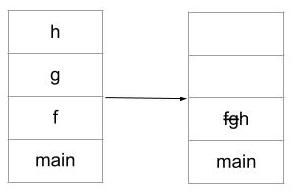
\includegraphics[width=0.3\textwidth]{tail_call}
			\caption{Tail call support}
			\label{fig:test}
		\end{figure}
		
		We can reuse stack frames!\\
		While this is arbitrary in the above case, it is key with recursion!\\
		A note: this is dangerous in C due to side effects, but we use Scheme purely functionally.
\end{enumerate}

\subsubsection*{Syntax}
\begin{lstlisting} [language=Lisp]
	; comment
	identifiers; string of ascii characters not beginning with number, '+', '-', '...', '->'
	;These are used for 3 things, all of which can be seen in the line:
		(let (x 'abc))
		; variables -- (x)
		; keywords --  (let)
		; symbol -- ('abc)
	(pa . ir)
	(l i s t); a pair chain ending with '() 
	#t #f ; booleans; ONLY #f is false
	"str\ning"
	#\c ; character
	'x ; data item x, non-evaluated
	`(f x (g ,y)) ; evaluates only y
\end{lstlisting}

\subsubsection*{Semantics}
\noindent Nearly everything in Scheme is represented by a function call.
\begin{lstlisting} [language=Lisp]
	; Format:
	(function arg1 arg2)
	; all elements are expressions evaluated left to right prior to call
 
	; Scheme provides a few standard functions:
	(cons x y); yields a pair (x, y)
	(car x); yields the first element of pair x
	(cdr x); yields the second element of pair x
	(eq? x y); yields #t iff x & y are the same object
	(eqv? x y); yields #t iff x & y have the same value
		(eqv? 5 5) ; -> #t
		(eq? 5 5); -> undefined (depends on compiler representation)
	(equal? x y); yields #t if x & y have the same recursively dereferenced value
	( = x y); yields #t iff x & y are numbers with equivalent values
	(list? x); yields #t iff x is a list
	(null? x); yields #t iff x is the empty list '()
	(eq? x '()) ; There is only one empty list, so this is equivalent
 
	; there are a few specific special cases:
	; (1)
	(quote x); yields x without evaluation
 
	;(2)
	(lambda FORMALS EXPRS); yields a function: FORMALS -> EXPRS(FORMALS)
	; we can allow any number of parameters:
	(lambda (FORMAL . ARGV) EXPRS); yields a lamba function w/ FORMAT+ arg count
	; binds parameter1 to FORMAL, rest as dotted list to ARGS; similarly
	(lambda . FORMAL EXPRS); 0+ parameter special case, since .() is an error
	; data is represented as (IMPROPERLIST . '())
		(list a b c); -> (a . (b . (c . ())))
		(cons a b); -> (a . b)
		'(a b); -> (quote . ((a . (b . ())) . ()))
	; thus we are "hacking" the representation
 
	; (3)
	(define NAME VALUE); binds evaluated NAME to VALUE (can be lambda expr)
	; though this can be used for constants, it is often for functions
	(define (NAME FORMALS) EXPRS); == (define NAME (lambda(FORMALS) EXPRS))
	; we can use this with the dot for very concise definitions:
		(define (list . x) x)
		(define (id x) x)
		(define (cons x y) x.y)
 
	; (4)
	(if TEST THEN ELSE); evaluate TEST; if #t THEN else ELSE
	; why is this necessary; couldn't we do it as a function? Like
		(define (funif test then else) #| flow control|#)
		(funif #t 97 26); -> 97
		(funif #t 0 0/0); -> ERROR
	; NO -- if must evaluate lazily rather than eagerly
	; we can use this to implement 'not'
		(define (funnot x) (if x #f #t)
 
	; (5)
	(and (E1 ... En)); yield #f on first failure, else last expression's value
	(or (E1 ... En)); yield first true, else #f
	; but wait, can't we just implement this with 'if'?
		(define (funand . args)
		  (if (null? args)
		    #t
		    (if (not ((car args))
		      #f
		     (funand (cdr args))))))
	; NO -- we again cannot prevent eager evaluation
 
	; there is another form that is tempting to include on this list:
	(let BINDINGS EXPRS); evaluate vals in BINDINGS, assign to vars, evaluate EXPRS
	; but this functions just like lambda; consider:
		(let ((x (+ 3 5))
		  (y (* 2 7)))
		  (+ (* x x) (* y y)))
	; is equivalent to
		((lambda (x y)
		  (+ (* x x) (* y y)))
		  (+ 3 5) (* 2 7))
	; thus 'let' can be thought of as "syntactic sugar"
	; it is included to allow our code to be written in evaluation order
\end{lstlisting}

\noindent Now we will write our canonical reverse function:
\begin{lstlisting} [language=Lisp]
	(define (reverse ls)
	  (if (null? ls)
	    ls
	    (append (reverse (cdr ls)) (list (car ls)))))
	; but unsurprisingly, this would be (N^2)
	; we then use a named let
	(define (reverse ls)
	  (let revapp ((ls ls) (a '())
	    (if (null? ls)
 	      a
	      (revapp (cdr ls) (cons (car ls) a)))))
	; this preserves execution order and lets us use easy tail recursion!
\end{lstlisting}
\noindent We use functional programming with Scheme, so set! is considered taboo, \\
\indent but there is an element even more controversial:

\subsubsection*{Continuations}
\noindent Proponents say they are the "essence of Scheme."\\
\noindent Opponents say they are too low level.\\
\noindent Professor Eggert likes them, but thinks simple ones are often too low level.\\
\\
What is a continuation?\\
\\
 Note that an interpreter always keeps track of:\\
 1. What to do next? (IP) ~~ \%rip\\
 2. What env to do it in? (EP) ~~ \%rbp/\%rsp\\
 A continuation packages these two things as a pair.\\
 Therefore the program can easily control flow!\\
\\
We can make a continuation at any time with call-with-current-continuation.\\
\\
 When we call (call/cc PROCS), the system:\\
 \begin{enumerate} [itemsep=0mm]
	\item Creates a continuation pointing at the return address of call/cc.
	\item Calls PROC with the continuation as a parameter.
	\item Returns whatever PROC returns
\end{enumerate}

\noindent How do we use a continuation? An example:
\begin{lstlisting} [language=Lisp]
	(define (product ls)
	  (call/cc
	    (lambda (break)
	      (let (prod ((ls ls))
		(if (null? ls)
		  1
		  (if (zero? (car ls))
		    (break 0)
		    (* (car ls) (prod (cdr ls))))))
	; we use a continuation to "escape" from a deeply nested recursion
\end{lstlisting}

\noindent This example allows us to “play with the program’s brain” with a “nonlocal goto”.\\
This is a common idea in many languages: consider exception handling\\
\begin{lstlisting} [language=Java]
	try {/* exception */} except(E e) {/* catching code */;}
\end{lstlisting}
We can do this with continuations in the following way:
\begin{enumerate} [itemsep=0mm]
	\item Create a continuation k.
	\item Give it to the main code.
	\item If k is used, we are back at the top level.
\end{enumerate}
\noindent We can use continuations in a more powerful way to jump back into a returned function!\\
A common usage for this is Green Threads — multithreading with one CPU.\\

 This is common in small, single core environments in the IoT.\\
 The basic idea:
 \begin{enumerate} [itemsep=0mm]
	\item Use continuations to switch from one thread to another.
	\item Cooperative scheduling with yield including continuation construction.\\
\end{enumerate}
\begin{lstlisting} [language=Lisp]
	; list of threads to run
	(define thread-list '())
	; add a thunk (no parameter call) to the thread list
	(define (new-thread thunk)
	(set! thread-list (append thread-list (list thunk))))
	; start a given thunk
	(define (start)
	  (let ((next-thread (car thread-list)))
	    (set! thread-list (cdr thread-list))
	    (next-thread)))
 	; give up the CPU
	(define (yield)
	  (call/cc
	    (lambda (k)
	      (new-thread (lambda() (k 42)))
	    (start)))))
	; usage:
	(new-thread (lambda() ((let (f (display "h") (yield)) (f))))
	(new-thread (lambda() ((let (f (display "e") (yield)) (f))))
	(new-thread (lambda() ((let (f (display "y") (yield)) (f))))
	(new-thread (lambda() ((let (f (newline) (yield)) (f))))
	(start) ; -> hey\nhey\nhey\n.........
\end{lstlisting}
\noindent This would traditionally be very hard to do in C but we have two ways of approaching it.\\
Note: C CODE\\
\begin{lstlisting} [language=C]
	#include <setjmp.h>
	// this library defines:
	  #typedef /*...*/ jmp_buf 
	  // a machine independent array == continuation
	  int setjmp(jmp_buf env); 
	  // uses %rip, %rsp to save to jmp_buf & return 0
	  _noReturn void longjmp(jmp_buf env, int val);
	  // puts VAL into %eax (return value) and jumps to jmp_buf w/ a continuation
	  // this effectively utilizes a try with a long jump ~= throw
	  // this is not as powerful as scheme -- we can only jump out 1 frame max
	  // -> we can do 'product' but not 'green-threads'
 
	// we have another more powerful version, but that makes it more controversial
	#include <wcontext.h>
	  // this library defines:
	  #typedef /*...*/ wcontext_t;
	  // another version of a continuation
	  int getcontext(wcontext_t *p);
	  // creates and stores a current continuation
	  int setcontext(wcontext_t const *p);
	  // resume from continuation *p
\end{lstlisting} \medskip
\noindent Scheme is a simple core language with an easy way to extend on syntax.\\
These are called syntax extensions, and we can use it to redefine ‘let’
\begin{lstlisting} [language=Lisp]
	(define-syntax let
	  (syntax-notes ()
	    ((let ((name val) ...) body1 body2 ...)
	      ((lambda (name) ...) body1 body2 ...) val ...))
		((let tag ((name val) ...) body1 body2 ...)
		  ((letrec ((tag (lambda (name ...) body1 body2 ...)))
		tag)
	      val ...))))
	; we could also redefine 'and'
	(define-syntax and
	  (syntax-rules ()
	    ((and) #t)
	    ((and e) e)
	    ((and e1 e2 ...)
	    (if e1 (and e2 ...) #f))))
	; usage:
	(and ((i 1) (< -10 i)) -> (if (< i 1) (< -10 i) #f)
	; clearly, we could also do this with 'OR', right?
	(define-syntax syn-or
	  (syntax-rules ()
	    ((syn-or) #f)
	    ((syn-or e) e)
	    ((syn-or e1 e2 ...) (if e1 e1 (or e2 ...))))
	; BUT this doesn't work -- consider:
	> (or (getenv "PATH") (getenv "PATH") "bin:/usr/bin")
	    (if (getenv "PATH") (getenv "PATH") ("/bin:/usr/bin"))
	; getenv is evaluated twice -- this is expensive and may have side effects!
	(define-syntax syn-or
	  (syntax-rules ()
	    ((syn-or) #f)
	    ((syn-or e) e)
	    ((syn-or e1 e2 ...)
	    (let ((x e1))
	    (if x x (or e2 ...))))))
	; but this has an even more subtle issue -- CAPTURE; consider:
	(let ((x "usr:/usr/bin"))
	  (or (getenv "PATH") x))
	; this would be transformed to:
	(let ((x "usr:/usr/bin"))
	  (let ((x getenv "PATH"))
	    (if x x (or x))))
	; Our macro expansion has captured x in a context it doesn't belong!
	; Scheme resolves this by resolving scope BEFORE macro expansion
	; These are called "hygienic macros", since they are "cleaner" than C
	; This doesn't require inter-compiler agreement since it is internal
\end{lstlisting} \medskip

\noindent Scope of identifiers in Scheme:
\begin{lstlisting} [language=Lisp]
	; most of the time, Scheme scope functions statically and like C
	(let ((x 3))
	  (let ((y 4))
	    (let ((x (+ y 1)))
	      (* x y))))
	; -> 20
	; BUT there are cases where this is not true
	(define (foo)
	  (let ((x 3))
	    (let ((x (+ x 5))
		   (y (+ x 2)))
		(* x y))))
	> (foo) ; 40
	; Scheme evaluates variables first to last, so we would expect 80 but get 40
	; Thus we can see the scope of a variable defined by 'let' does not extend
	; into the definitions of other parallel defined variables
	; Why is this? Because of the equivalence of 'let' to 'lambda'!
	(define (foo)
	  (lambda (x)
	    ((lambda (x y) (* x y))
	    (+ x 5) (+ x 2))
	  3))
	; Scheme uses the 'let*' keyword for sequential definition:
	(define (foo)
	  (let* ((x 3))
		  (y (+ x 2)))
	  (* x y)))
	> (foo) ; 15
\end{lstlisting}

\end{document}